\documentclass[a4paper,12pt,english]{all-in-one} %% TWOSIDE
\usepackage{amsmath} 
\usepackage{newtxmath}
\usepackage{multicol}
\usepackage{lipsum}
\usepackage{subfig}
\usepackage{listings}
\usepackage[hidelinks]{hyperref}
\renewcommand\theequation{\arabic{equation}}
\newcommand\tab[1][1cm]{\hspace*{#1}} 

\doctitle{Modern Physics Laboratory }
\docsubtitle{Cavendish Experiment} % Experiment name here

\makeatletter
\title{{\large\textit{Modern Physics Laboratory | PHYS-461}}\\[0.5cm]{\Huge\color{gray}\textsc{\@docsubtitle}}}
\makeatother

\author{\textbf{Cordney Nash}  }
\date{December 2, 2024}
\footext{}



\begin{document}

\begin{titlepage}
\maketitle\vfill
\end{titlepage}
\newpage 


\section*{Introduction}
{
The objective of this lab experiment was to investigate forces, specifically the gravitational force and we did this by replicating the Cavendish Experiment to determine an experimental universal gravitational constant ($G$). This was achieved using a torsion balance, a sophisticated frame to hold it, lasers, and lead ($Pb$) masses. This experiment functions by understanding the pull two masses have on each other. Additionally, by knowing the dimensions of the setup, a mathematical relationship can be derived to calculate the value of $G$
}

\begin{figure}[tbh]
    \centering
    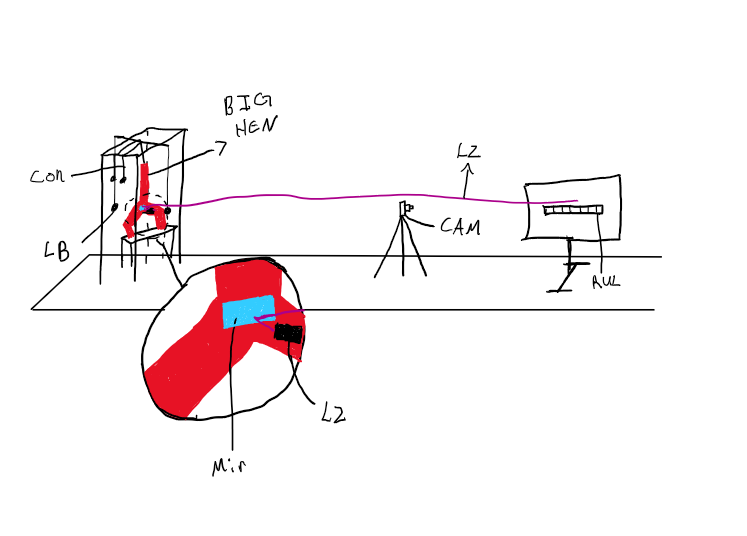
\includegraphics[width=0.8\linewidth]{7-cavendish/overleaf/droc/images/cavendish_schem.PNG}
    \caption{ \scriptsize{ controls for the placement of the lead balls (Con), lead balls (LB), pendulum mirror (Mir), laser (LZ), camera (CAM), and ruler (RUL). Henry (BIG HEN) is the frame that holds the torsion balance measurer and two small tungsten masses.
    }}
    \label{fig:cavndish-diagram}
\end{figure}

% \begin{multicols}{2}

\section*{Theory \& Procedure}
{
At the heart of this experiment is a gravitational torsion balance, a special device that allows us to negate Earth's gravity while allowing for the precise measurement of exceptionally delicate forces. The torsion balance responds to a gravitational interaction by proportionally twisting a beryllium copper ribbon. In this situation that force is due to the gravitational pull two sets of large and small masses have on each other. That gravitational force is represented by:
\begin{equation}\label{eq: Force_grav}
    F_{grav} = G\frac{Mm}{r^2}
\end{equation}
where M and m are the mass of the large and small masses respectively, and
r is the distance between their centers. Eq:\eqref{eq: Force_grav} is important because if we know that the torque in the torsion wire is:
\begin{equation}\label{eq:torsion}
    \tau = 2Fd
\end{equation}
we can substitute and get:
\begin{equation}\label{eq:torsion_plus_grav}
    \tau = 2G\frac{Mm}{r^2}d
\end{equation}

where d is the distance to the pivot point in the balance device. Eq:\eqref {eq:torsion_plus_grav} provides a direct relationship between the torsion in the balance as a function of the applied force $F_{grav}$. To further interpret this experiment, we must understand that across both ends the torque is $\Delta\tau = 2\tau$.

It is also important to know that when studying torsion motion, this relationship for torque $\tau$:
\begin{equation}\label{eq:change_in_torque}
    \Delta\tau = -k\Delta\theta 
\end{equation}
can be shown, as $\theta$ is the angle the head is reflected by and $k$ is a torsion constant. The period associated with this torsion motion is:
\begin{equation}\label{eq:toursion_perios}
    t = 2\pi\sqrt{\frac{2md^2}{k}}
\end{equation}

\begin{equation}\label{eq:toursion_perios}
    2\tau = \Delta\tau
\end{equation}

In all, knowing all of this, equating Eq:\eqref{eq:change_in_torque} with $2\tau$ and taking into account the period $t$, we can end up at a relationship between G and known experimental parameters:
\begin{equation}\label{eq:grav_constant}
   G = \frac{2\pi^2r^2\lambda}{Mt^2}
\end{equation}
where $\lambda \equiv d\Delta\theta$ and equals $4.004E^{-03}$ for trial 1 and $4.114E^{-03}$ for trial 2.

To initiate the experiment, ideally, the weights are rotated to one extreme for 90 minutes, which is around 5 full oscillations, causing the torsion balance to twist. After the time is up at this extreme point, we rotate the large masses to the other extrema for another 90 minutes. When collecting data we tracked laser deflections off a board sitting at $\sim$5.05 $m$ away from Henry. In our case, we recorded data by using a camera set to 1 picture every 20 seconds, which was positioned on the board. When done we combine the images into one singular video for further use.


}

\begin{figure}[h]
    \centering
    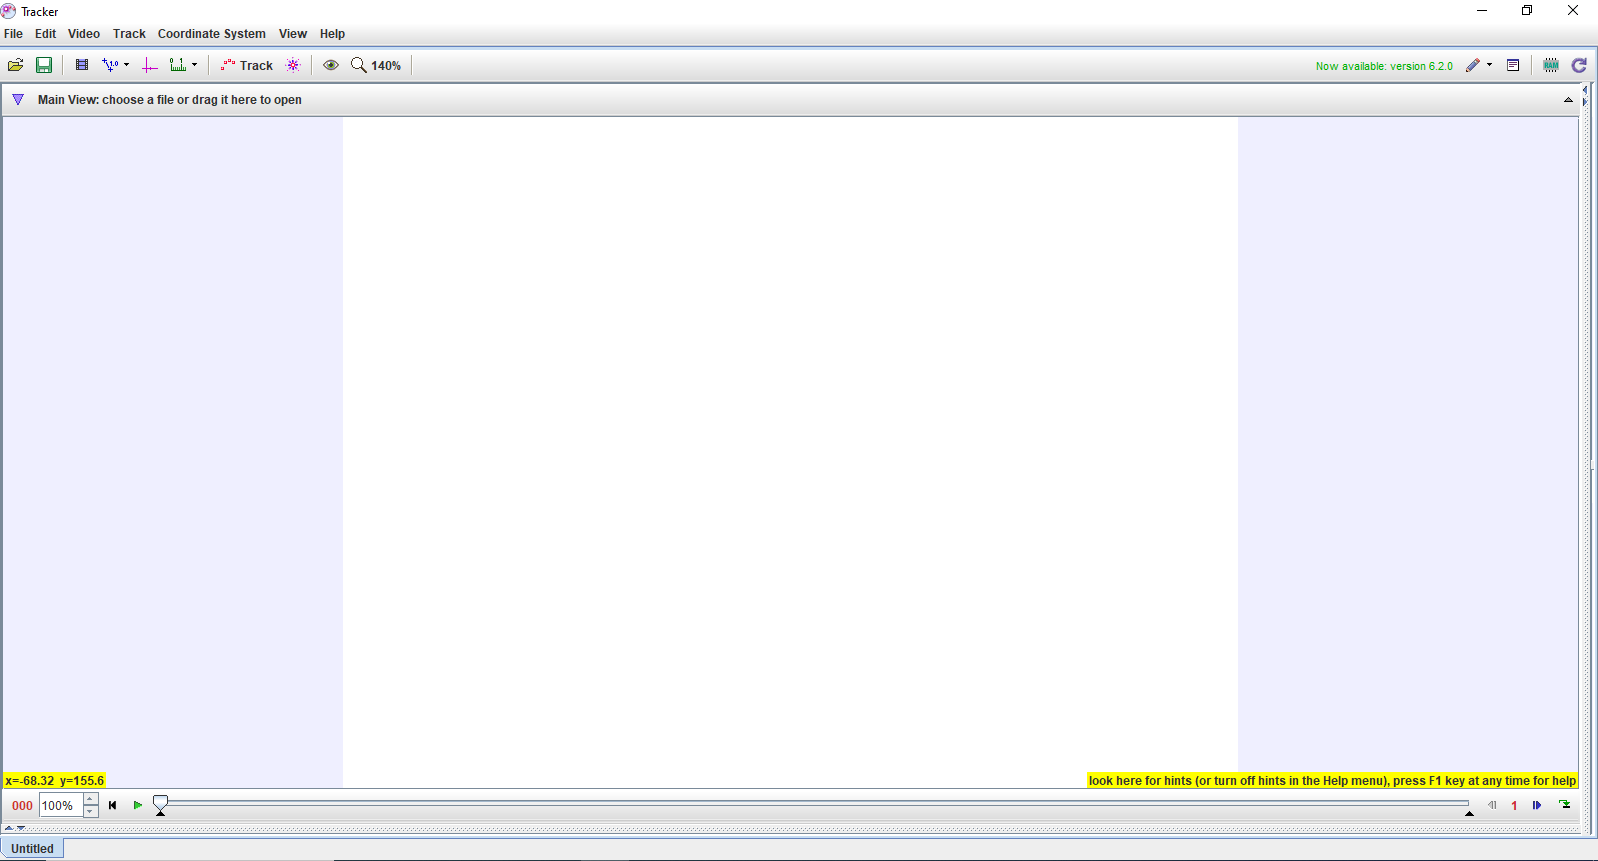
\includegraphics[width=1.0\linewidth]{7-cavendish/overleaf/droc/images/Capture.PNG}
    \caption{ A screenshot of the Tracker software.}
    \label{fig: cavendish tracker}
\end{figure}

\section*{Analysis \& Results}
{
In this experiment, we utilize a method similar to "Measurement by Equilibrium Position," as described in the torsion balance manual. We position two large masses at two extremes and by using a software called "Tracker" we measure the equilibrium point after what can be described as dampened oscillations. 

The Tracker software can help us determine this equilibrium position by tracking the horizontal movement of the reflected laser through the video assembled earlier. The software calculates the position as a function of time and prints out what resembles a dampened sine wave. By using tools found in the Tacker software and knowing the physical properties of the system we can find:

\noindent
\\
\\
\begin{center}
{\begin{tabular}{c|c}
t & 1034.506571 seconds (s) $\pm$ 4.091925927 s\\
M & 22.231 kilograms (kg) $\pm$ 2 kg\\
$\lambda$ & $4.059E^{-03}$ meters (m) $\pm$ 0.00007824381571 m\\
r & 0.14763 meters $\pm$ 0.0381 m\\
\end{tabular}
}
\end{center}

\noindent
This table shows the average values of the parameters used in both trials to find $G$. But, I must note that the errors given for M and r are merely estimated errors I deemed appropriate. From each run, we can average the calculated $G$ by using Google Sheet's AVERAGE function and find a standard deviation by using their STD function. We get:

\begin{center}
{\begin{tabular}{c|c}
$G$ & $7.354E^{-11} \pm 8.36E^{-13} \quad [Nm^2/kg^2]$ 
\end{tabular}
}
\end{center}
% \begin{equation}\label{eq:grav_constant_plus_constant}
%    G = \frac{2\pi^2(0.14763)^2(1.116E^{-02})}{(22.231)(1031.613143)^2\frac{1}{0.998}} = 2.033E^{-10} \quad [Nm^2/kg^2]
% \end{equation}
% where $\frac{1}{0.998}$ is a correction factor. 
This averaged value is within 5\% of the accepted value $G = 6.67E^{-11} Nm^2/kg^2$. 

We believed that possible sources of error may have been due to setting the extrema position slightly off at the beginning. If this offset is larger than $r$ this can cause a weak pull from the two masses. Other sources of error, although small, maybe the mass of an elevator on the other side of a wall adjacent to Henry. The constant movement of this mass could cause slight deviations in the force the torsion wire picks up, thus potentially propagating an error through calculations. 

}
% \end{multicols}

\section*{Summary}
{
This experiment aimed to replicate the Cavendish Experiment to determine the universal gravitational constant ($G$) by analyzing the gravitational attraction between two sets of masses using a torsion balance. By tracking laser deflections and calculating the equilibrium position after dampened oscillations, my lab partner and I derived G using a mathematical relationship between torque and gravitational force. Despite its obscure appearance, the experiment demonstrated the effectiveness of the Cavendish method for accurately measuring 
$G$ and provided insights into the challenges of precise measurements of gravity-related physics.
}




\end{document}